\subsection{Query Expansion and Index Analysis}
\textbf{Student Name: }Marcelo Almeida \textbf{Student ID:} 0877394 \\
Introduction

\subsubsection*{Motivation}
In Information Retrieval (IR) a query is a way to materialize in a sentence (or word) the user's information needs. This means that if the query is poorly crafted, the user probably will not be able to retrieve the wanted content. One way to address the problem is to expand  the query by adding related terms, retrieving more results that might satisfy the information need. Here our goal is to do so relying on a dictionary, meaning that each query term will be mapped to a set of related terms and those terms will also be used to fetch the content from the database. Besides, the user expects this query to work fast, and that is usually done through an index. It is good to store this index occupying the least storage space as possible. We will also make a brief study of two index formats.

\subsubsection*{Problem formulation}
Given a query, we want to search for other words that have the same meaning of those used in the query. We also want to analyze how many KB the index occupies in known index implementations.


\subsubsection*{Approach}
Our first choice was to use an open source library for Python called NLTK (Natural Language ToolKit). It is built over Wordnet, which contains a well known set of synonyms, and have been in development for years. With this package we implemented the query expansion and also a way of using user feedback to change the meaning of the presented set of synonyms (relevance feedback). Unfortunately later we decided to build the interface using Java and we were not able to integrate these two programs. It was necessary to recreate the query expansion program in Java and we did so using a (Wordnet based) package from Apache Lucene project. This package did not offer the same functionality as the Python one and because of that, along with the time constraints, we could not add user feedback. In the end, the query expansion presents more terms related to those already used in the query.
 
For the study of the space usage we used two different types of index. First, using a Weka filter we converted the Reuters 50x50 dataset \cite{reuters50x50} to a vector space representation and built the adjacency matrix, represented by a CSV file. This file was rather sparse, as partially shown in Figure \ref{adjacency_matrix}.
\begin{figure}[h!]
 \centering
 \label{adjacency_matrix}
   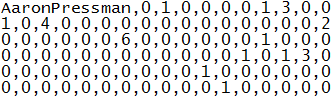
\includegraphics[width=0.5\textwidth]{adjacency_matrix.png}
 \caption{Only part of the adjacency matrix already shows its sparseness.}
\end{figure}

After that we created a Python program to build the inverted index of the same dataset (in three different ways, one of them using NLTK library to deal with the stopwords) and the comparison of all representations can be seen in the table \ref{space_comparison}).

\begin{table}[ht]
	\label{space_comparison}
	\centering
	\caption{Different types of index representations and their required storage space.}
    \begin{tabular}{| p{7cm} | p{3cm} |}
    	\hline
		Representation & Space requirements (KB) \\ \hline
		Usual adjacency matrix (CSV file) & 53.413 \\ \hline
		Inverted index without token normalization and \\ without removing stop words & 5.411 \\ \hline
		Inverted index without token normalization but \\ removing stop words & 4.785 \\ \hline
		Inverted index with token normalization (lowercase only) \\ and removing stop words & 4.567 \\ \hline
    \end{tabular}
\end{table}

\subsubsection*{Evaluation}
For the query expansion, we ran the same query with and without the expansion feature and we noticed that without context evaluation to use along with the dictionary it might be hard to know if the new (expanded) query means what the user wants. For example, a query for $\{mobile\}$ was expanded to $\{mobile, fluid, nomadic, peregrine, roving, wandering\}$. We get more results with the new query, but they will not be relevant to a user searching for mobile phone. It was not possible to calculate the recall, since we did not know how many documents were relevant (our database is too big for that evaluation). Regarding the precision, it would depend on the particular interest of the user. For the example above, if phone was the information need, the precision would be small. However, if it was movement, then it would be bigger.
For the index evaluation, it is very clear from the results presented in table \ref{space_comparison} that the inverted index is, indeed, a good choice as a data structure, occupying less than $ 9\% $ of the space used by the adjacency matrix.

\subsubsection*{Few observations}
We thought of a few possible different improvements that could also be interesting for query expansion. First, we could add different (smaller) weights for additional terms. That would make the original query more relevant but would still give a different result set. Second, instead of expanding the query without telling the user, we could show both the results for the query and also the other possible terms. Third (disregarding the dictionary), we could retrieve the results for the user’s query and extract the top keywords to show as suggestions. Since we did not intend to implement these ideas in the beginning and because of that they didn't fit in our timeframe.
